\documentclass[../ZF_SWEN1.tex]{subfiles}

\begin{document}

\begin{itemize}
	\item Gesamtheit der wichtigsten Entwurfs-Enscheidungen.
	\begin{itemize}
		\item Programmiersprachen, Plattformen
		\item Aufteilung: Teilsysteme, Bausteine, Schnittstellen
		\item Veratnwortlichkeiten und Abhängigkeiten der Teilsysteme
		\item Basis-Technologie oder Frameworks (z.B Java EE)
		\item Besondere Massnahmen um Anforderungen zu erfüllen
	\end{itemize}
	\item Grundlagen
	\begin{itemize}
		\item Anforderungen (vorallem nicht-funktionale)
		\item Systemkontext mit Schnittstellen
	\end{itemize}
	\item Top Level View (das grosse Ganze)
\end{itemize}

\subsubsection{Übersicht Buisiness Analyse vs Architektur vs Entwicklung}

\paragraph{Business Analyse}
\begin{itemize}
	\item Domänenmodell
	\item Kontext Diagramm
	\item Requirements
	\begin{itemize}
		\item Liste Stakeholder
		\item Vision
		\item Funktionale Anforderungen:
		\begin{itemize}
			\item Use Cases / User Stories
		\end{itemize}
		\item Nicht funktionale Anforderungen:
		\begin{itemize}
			\item Supplementary Specification
		\end{itemize}
		\item Randbedingungen
		\item Glossar
	\end{itemize}
\end{itemize}

\paragraph{Architektur}
\begin{itemize}
	\item Logische Architektur
\end{itemize}

\paragraph{Entwicklung}
\begin{itemize}
	\item Use Case / User Story Realisierung
	\item Anwendung GRASP
	\item DCD - Design-Klassen-Diagramm
	\item Interaktionsdiagramme
	\item Programmierung
	\item Erstellen der Unit-/Integrations-Tests
\end{itemize}

\begin{figure}[H]
\centering				\includegraphics[width=0.3\textwidth] {Resources/Images/Übersicht.png}
\caption{\label{fig:Übersicht}Übersicht}
\end{figure} 


\subsubsection{Wie entstehen Architekturen}

\begin{figure}[H]
\centering				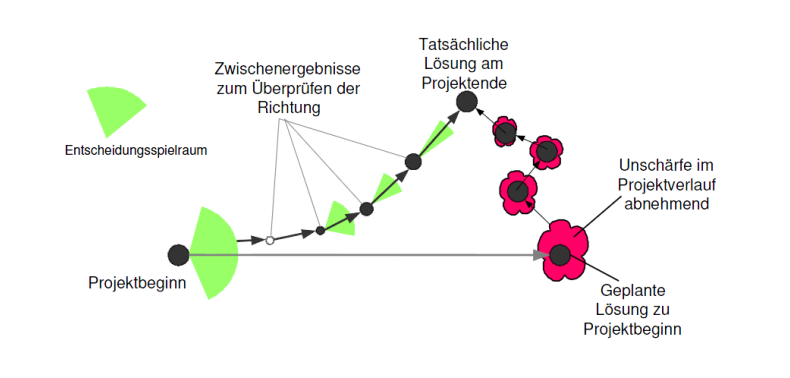
\includegraphics[width=0.3\textwidth] {Resources/Images/ArchitekturEntstehung.png}
\caption{\label{fig:ArchitekturEntstehung}ArchitekturEntstehung}
\end{figure} 

\paragraph{Architektur aus Anforderungen ableiten}

\begin{itemize}
	\item Muss heutige und zukünftige Anfroderungen erfüllen können
	\item Aufgabe Architekturanalyse
	\begin{itemize}
		\item Analyse funktionale und nicht funktionale Anforderungen und deren Konzsequenzen
		\item  Berücksichtigung Randbedingung und zukünftige Veränderungen
		\item Qualität, Stabilität der Anforderungen prüfen
		\begin{itemize}
			\item Lücken in Anforderungen aufdecken
		\end{itemize}
	\end{itemize}
\end{itemize}


\title{Twin peak Model}
\begin{figure}[H]
\centering				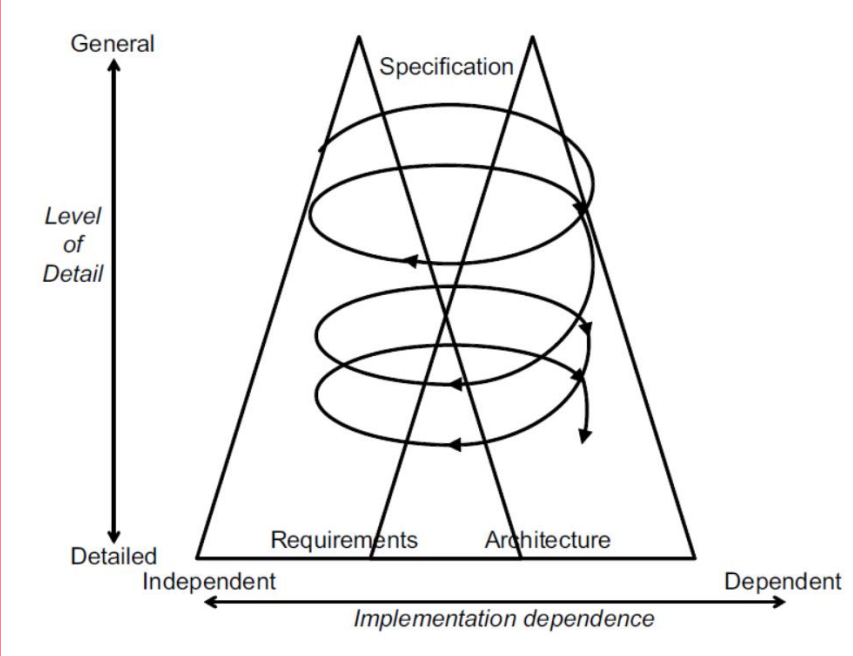
\includegraphics[width=0.3\textwidth] {Resources/Images/TwinPeak.png}
\caption{\label{fig:TwinPeak}TwinPeak}
\end{figure}

\title{Entwurfsentscheidungen}
\begin{figure}[H]
\centering				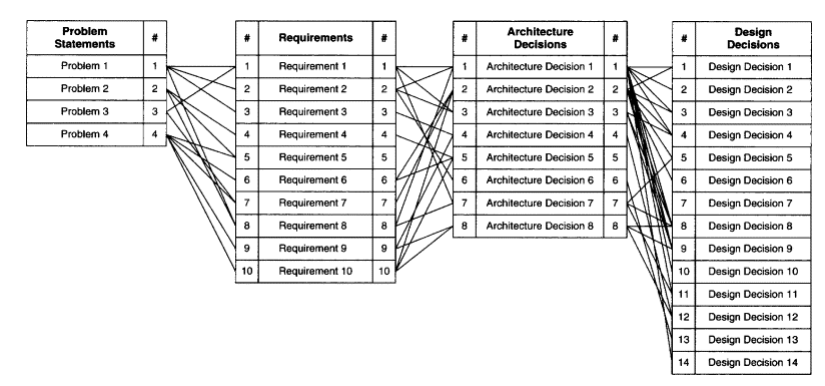
\includegraphics[width=0.3\textwidth] {Resources/Images/EntwurfsEntscheidungen.png}
\caption{\label{fig:EntwurfsEntscheidungen}EntwurfsEntscheidungen}
\end{figure}

\title{Nichtfunktionale Anforderungen}
\begin{figure}[H]
\centering				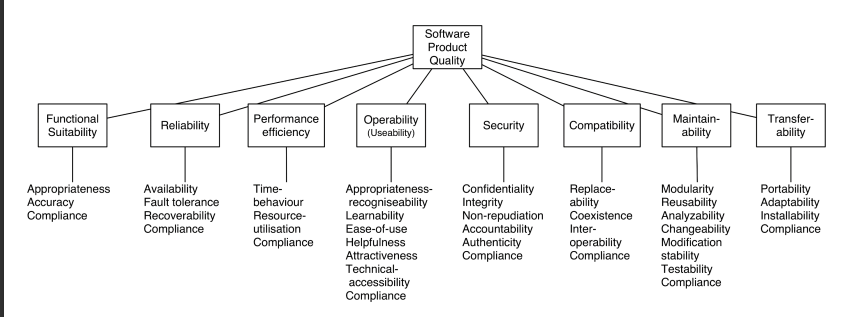
\includegraphics[width=0.3\textwidth] {Resources/Images/NichtfunktionaleAnforderungen.png}
\caption{\label{fig:NichtfunktionaleAnforderungen}NichtfunktionaleAnforderungen}
\end{figure}

\subsection{Modulkonzept}
\begin{itemize}
	\item Modul(Baustein, Komponente):
	\begin{itemize}
		\item Autarkes Teilsystem
		\item Klare, minimale Schnittstelle gegen Aussen
		\item Software-Modul enthält alle Funktionen und Datenstrukturen
		\item Modul: Paket, Programmierkonstrukt, Library, Komponente, Service
	\end{itemize}
	\item Konzept in allen Ingenierdisziplinen angwendet
	
\end{itemize}

\begin{multicols}{2}
\title \textcolor {orange} {Schnitstellen Kapselung und Austauschbarkeit}
\begin{figure}[H]
\centering				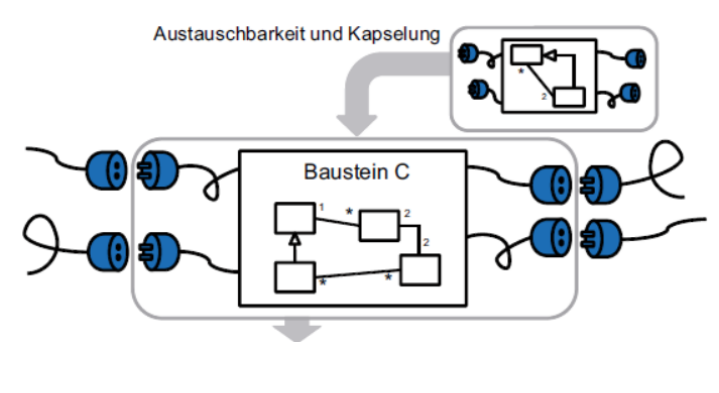
\includegraphics[width=0.3\textwidth] {Resources/Images/Schnittstellen.png}
\caption{\label{fig:Schnittstellen}Schnittstellen}
\end{figure}

\columnbreak

\title \textcolor {orange}{Prinzip modularen Strukur}
\begin{figure}[H]
\centering				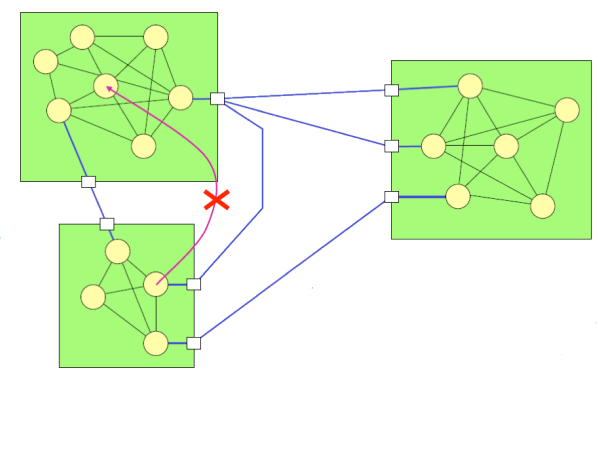
\includegraphics[width=0.3\textwidth] {Resources/Images/ModularenStruktur.png}
\caption{\label{fig:ModularenStruktur}ModularenStruktur}
\end{figure}


\end{multicols}

\subsubsection{Messung der Güte einer Modularisierung}
\begin{itemize}
	\item Kohäsion (Stärke inneren Zusammenhangs)
	\begin{itemize}
		\item \colorbox{yellow!30}{schlecht:} zufällig, zeitlich
		\item \colorbox{yellow!30}{gut:} funktional, objektbezogen
		\item je \textcolor {blue}{höher} Kohäsion innerhalb Modul, desto \textcolor {blue} {besser} die Modularisierung
	\end{itemize}
	\item Kopplung (Abhängigkeit zwischen 2 Modulen)
	\begin{itemize}
		\item \colorbox{yellow!30}{schlecht:} Globale Kopplung
		\item \colorbox{yellow!30}{akzeptabel:} Datenbereichskopplung (Referenzen auf gemeinsame Daten)
		\item \colorbox{yellow!30}{gut:} Datenkopplung (alle Daten werden beim Aufruf der Schnittstelle übergeben)
		\item Je \textcolor {blue}{geringer} die wechselseitige Kopplung desto \textcolor {blue}{besser} die Modularisierung
	\end{itemize}
\end{itemize}

\title Clean Architecture
\begin{figure}[H]
\centering				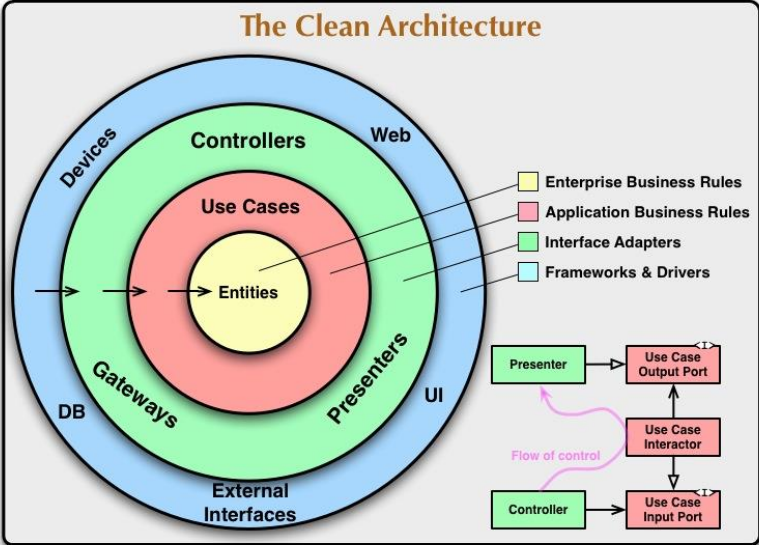
\includegraphics[width=0.3\textwidth] {Resources/Images/CleanArchitecture.png}
\caption{\label{fig:CleanArchitecture}CleanArchitecture}
\end{figure}

\begin{itemize}
	\item Unabhängikeit:
	\begin{itemize}
		\item von Framework
		\item voneinander getestet werden
		\item von UI
		\item von DB
	\end{itemize}
\end{itemize}


\subsection{Architektur Beschreiben}

\textbf{Aufgeteilt in Views: \\}

\begin{itemize}
		\item Logical View
		\begin{itemize}
			\item Funktionalität gegen aussen
			\item Aspekte: 
			\begin{itemize}
				\item Schichten
				\item Subsysteme
				\item Pakete
				\item Frameworks
				\item Klassen
				\item Interfaces
			\end{itemize}
			\item \colorbox{yellow!30}{UML:}
			\begin{itemize}
				\item Systemsequenzdiagramme
				\item Interaktionsdiagramme
				\item Klassendiagramm
				\item Zustandiagramme
			\end{itemize}
		\end{itemize}
\end{itemize}

\begin{itemize}
	\item Process View
	\begin{itemize}
			\item Wo und wie im System
			\item Aspekte: 
			\begin{itemize}
				\item Prozesse
				\item Threads
				\item Wie Anforderungen erreicht
			\end{itemize}
			\item \colorbox{yellow!30}{UML:}
			\begin{itemize}
				\item Klassendiagramme
				\item Interaktionsdiagramme
				\item Aktiviitätsdiagramme
				\end{itemize}
		\end{itemize}
	
\end{itemize}

\begin{itemize}
	\item Development View (Implementation View):
	\begin{itemize}
			\item Wie Struktur umgesetzt
			\item Aspekte: 
			\begin{itemize}
				\item Source Code
				\item Executables
				\item Artefakte
			\end{itemize}
			\item \colorbox{yellow!30}{UML:}
			\begin{itemize}
				\item Paketdiagramme
				\item Komponentendiagramme
				\end{itemize}
		\end{itemize}	
\end{itemize}


\begin{itemize}
	\item Physical View (Deployment View)
	\begin{itemize}
			\item Auf welcher Infrastruktur wird System ausgeliefert /betrieben
			\item Aspekte: 
			\begin{itemize}
				\item Prozessknoten
				\item Netzwerke
				\item Protokolle
			\end{itemize}
			\item \colorbox{yellow!30}{UML:}
			\begin{itemize}
				\item Deployment Diagram
			\end{itemize}
		\end{itemize}
\end{itemize}


\begin{itemize}
	\item +1 View: Scenarios (Use Cases)
	\begin{itemize}
			\item Wichtigste Use Cases und ihre nicht funktionale Anforderungen? Wie umgesetzt?
			\item Aspekte: 
			\begin{itemize}
				\item Architektonisch wichtige UCs
				\item deren nichtfunktionale Anforderungen
				\item deren Implementation
			\end{itemize}
			\item \colorbox{yellow!30}{UML:}
			\begin{itemize}
				\item UC-Diagramm
				\item Systemsequenzdiagramme
				\item UC-Realisierungen
			\end{itemize}
	\end{itemize}
\end{itemize}

\begin{itemize}
	\item Daten-Sicht
	\item Sicherheit
\end{itemize}

\title Logische Architektur vs Physikalische Architeckur

\begin{multicols}{2}
\begin{figure}[H]
\centering				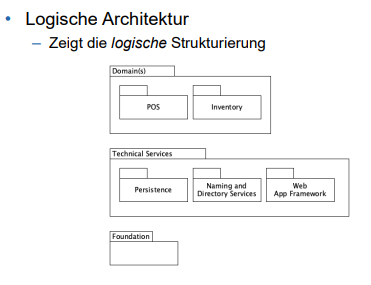
\includegraphics[width=0.3\textwidth] {Resources/Images/LogischeArchitektur.png}
\caption{\label{fig:LogischeArchitektur}LogischeArchitektur}
\end{figure}

\columnbreak

\begin{figure}[H]
				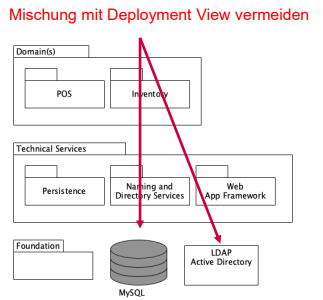
\includegraphics[width=0.3\textwidth] {Resources/Images/VermeidungArch.png}
\caption{\label{fig:VermeidungArch}VermeidungArch}
\end{figure}

\end{multicols}

\begin{figure}[H]			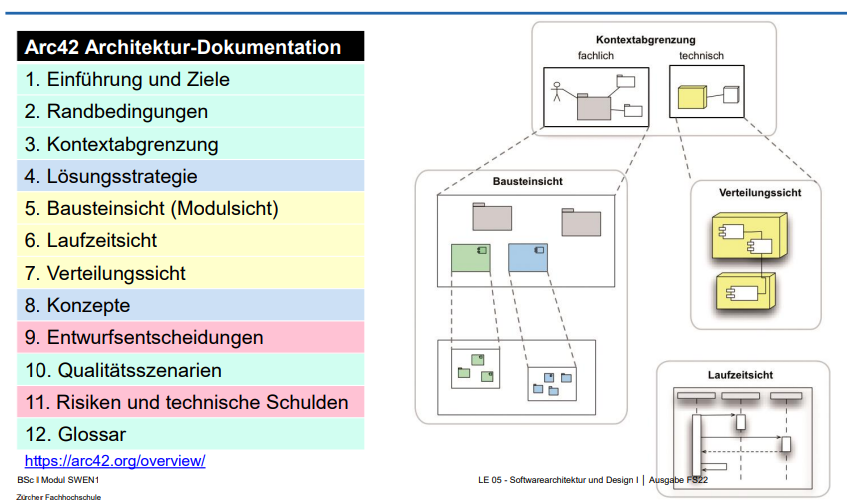
\includegraphics[width=0.3\textwidth] {Resources/Images/Arc42.png}
\caption{\label{fig:Arc42}Arc42}
\end{figure}

\subsection{UML-Paketdiagramme}

\begin{itemize}
	\item Mittel, zum Teilsysteme zu definieren
	\item Mittel zur Gruppierung von Elementen
	\item Paket enthält Klassen und andere Pakete
	\item Abhängigkeit zwischen Paketen
\end{itemize}



\subsection{Verteilungsdiagramm} 

\begin{itemize}
	\item Darstellung Verteilung von Komponenten auf Rechenknoten mit Abhängigkeiten, Schnittstellen und Verbindungen
	\item Statische Modellierung
\end{itemize}




\subsection{Ausgewählte Architekturpatterns}

\begin{table} [H]

\begin{tabular}{l|l}

\colorbox{green}{\textbf{Pattern}} & \colorbox{green}{\textbf{Beschreibung}}

\\\hline
\textbf{Layered Pattern} & Strukturierung eins Programms in Schichten\\
\hline
\textbf{Client-Server Pattern} & Server stellt Services für mehrere Clients zur Verfügung\\
\hline
\textbf{Master-Slave Pattern} & Master verteilt Arbeit auf mehrere Slaves\\
\hline
\textbf{Pipe-Filter Pattern} & Verarbeitung einses Datenstroms (filtern, zuordnen, speichern)\\
\hline
\textbf{Broker Pattern} & Meldungsvermittler zwischen verschiedenen Endpunkten \\
\hline
\textbf{Event-Bus Pattern} & Datenquellen publizieren Meldungen an einen Kanal auf dem Event-Bus.\\ &Datensenken abonnieren einen bestimmten Kanal\\
\hline
\textbf{MVC Pattern} & Ineraktive Anwendung in 3 Komponenten aufgeteilt:\\
& -Model \\
& -View - Informationsanzeige \\
& -Controller - Verarbeitung Benutzereingabe
\end{tabular}
\end{table}


\subsubsection{Layered Pattern}
\begin{multicols}{2}
\begin{itemize}
	\item Je weiter unten, desto allgemeiner
	\item Je höher, desto anwendungs-spezifischer
	\item Zuoberst ist das Benutzerinterface
\end{itemize}

\textbf{Kopplung von oben nach unten} \textcolor {red} {NIE} von unten nach oben.

\columnbreak

\begin{figure}[H]			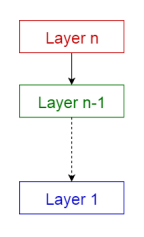
\includegraphics[width=0.3\textwidth] {Resources/Images/LayeredPattern1.png}
\caption{\label{fig:LayeredPattern1}LayeredPattern1}
\end{figure}

\end{multicols}

\pagebreak

\title{Anrufszenarien}

\begin{multicols}{2}

\begin{figure}[H]			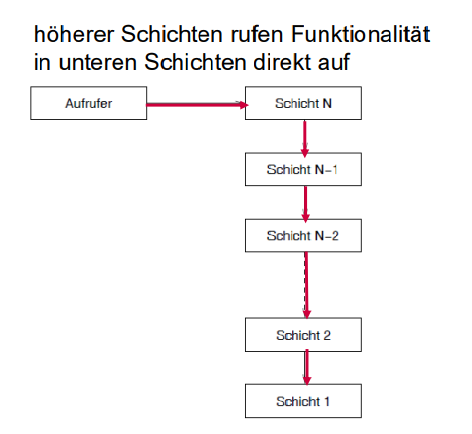
\includegraphics[width=0.3\textwidth] {Resources/Images/AnrufSzenarienH.png}
\caption{\label{fig:AnrufSzenarienH}AnrufSzenarienH}
\end{figure}


\columnbreak


\begin{figure}[H]			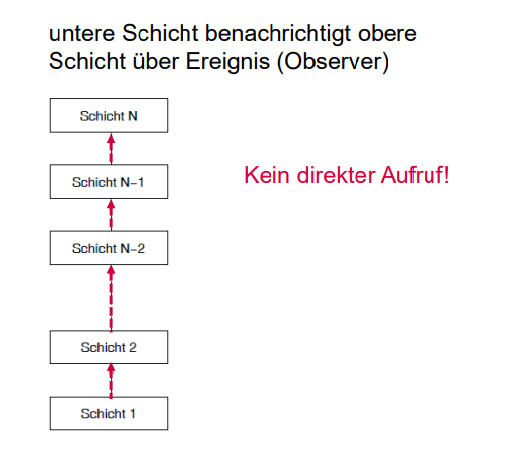
\includegraphics[width=0.3\textwidth] {Resources/Images/AnrufSzenarienObserver.png}
\caption{\label{fig:AnrufSzenarienObserver}AnrufSzenarienObserver}
\end{figure}

\end{multicols}


\begin{multicols}{2}
	\begin{itemize}
		\item UI
		\begin{itemize}
			\item Presentation, Windows, Dialoge, Reports, WEB, Mobile
		\end{itemize}
		\item Application
		\begin{itemize}
			\item Requests von UI Layer, Workflow, Sessions
		\end{itemize}
		\item Domain
		\begin{itemize}
			\item Requests von Application Layer, Domain Rules, Services
		\end{itemize}
		\item Business Infrastructure
		\begin{itemize}
			\item Low level business Services (z.B CurrencyConverter)
		\end{itemize}
		\item Technical Services
		\begin{itemize}
			\item Persistence, Security, Logging
		\end{itemize}
		\item Foundation
		\begin{itemize}
			\item Datenstrukturen, Threads, Dateien, Netwerk IO
		\end{itemize}
	\end{itemize}
\columnbreak

\begin{figure}[H]			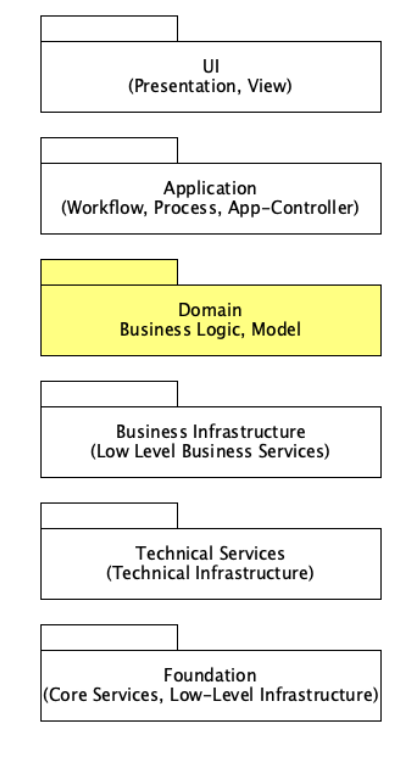
\includegraphics[width=0.3\textwidth] {Resources/Images/LayeredPattern2.png}
\caption{\label{fig:LayeredPattern2}LayeredPattern2}
\end{figure}

\end{multicols}


\subsubsection{Client-Server}

\begin{multicols}{2}
	\begin{itemize}
		\item 1 Server und mehrere Clients		
		\item 1 Server stellt einen oder mehrere Services zur Verügung		
		\item Client macht Request zum Server		
		\item Server sendet Response zurück		
	\end{itemize}
\columnbreak

\begin{figure}[H]			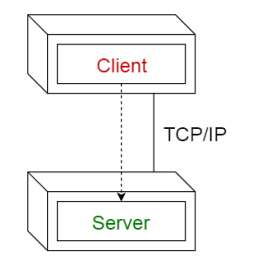
\includegraphics[width=0.3\textwidth] {Resources/Images/ServerClient.png}
\caption{\label{fig:ServerClient}ServerClient}
\end{figure}

\end{multicols}

\subsubsection{Master-Slave Pattern}

\begin{multicols}{2}
	\begin{itemize}
		\item Master verteilt die Aufgaben auf mehrere Slaves	
		\item Slaves führen Berechnungen aus und senden Ergebnis zum Master
		\item Maseter berechnet Endergebnis		
	\end{itemize}
\columnbreak

\begin{figure}[H]			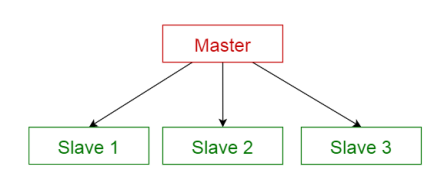
\includegraphics[width=0.3\textwidth] {Resources/Images/MasterSlave.png}
\caption{\label{fig:MasterSlave}MasterSlave}
\end{figure}

\end{multicols}

\subsubsection{Pipe-Filter Pattern}

\begin{multicols}{2}
	\begin{itemize}
		\item Verarbeitung von Datenströmen (Linux Pipe, RxJS Observable Streams, Java Streams,...)
		\item Verarbeitungsschritt durch Operator wie Filter, Maper, etc. umgesetzt
	\end{itemize}
\columnbreak

\begin{figure}[H]			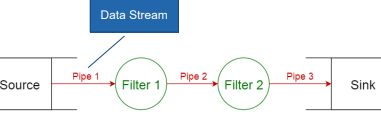
\includegraphics[width=0.3\textwidth] {Resources/Images/PipeFilter.png}
\caption{\label{fig:PipeFilter}PipeFilter}
\end{figure}

\end{multicols}


\subsubsection{Broker Pattern}
\begin{multicols}{2}
	\begin{itemize}
		\item verteilte Systeme mit entkoppelten Subsysteme zu koordinieren
		\item Broker(Vermittler) ermittelt Kommunikation zwischen einem Client und dem entspr. Subsystem
		\item Bsp.: Message Broker
	\end{itemize}
\columnbreak

\begin{figure}[H]			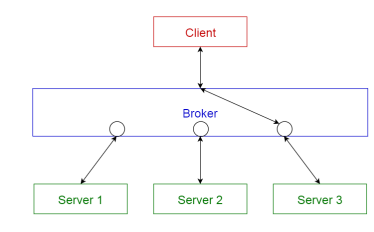
\includegraphics[width=0.3\textwidth] {Resources/Images/BrokerPattern.png}
\caption{\label{fig:BrokerPattern}BrokerPattern}
\end{figure}

\end{multicols}

\subsubsection{Event-Bus Pattern}
\begin{multicols}{2}
	\begin{itemize}
		\item 4 Hauptkomponenten:
		\begin{enumerate}
			\item EventSource
			\item Eventlistener
			\item Channel
			\item Event Bus
		\end{enumerate}
		\item \colorbox{blue!30}{Event Sources} publizieren Meldungen zu einem bestimmten \colorbox{blue!30}{Kanal} auf dem \colorbox{blue!30}{Event Bus}
		\item \colorbox{blue!30}{EventListeners:}
		\begin{itemize}
			\item Melden sich für bestimmte Events an
			\item werden informiert, sobald entsprechende Meldungen auf dem \colorbox{blue!30}{Kanal} befinden
		\end{itemize}
	\end{itemize}
\columnbreak

\begin{figure}[H]			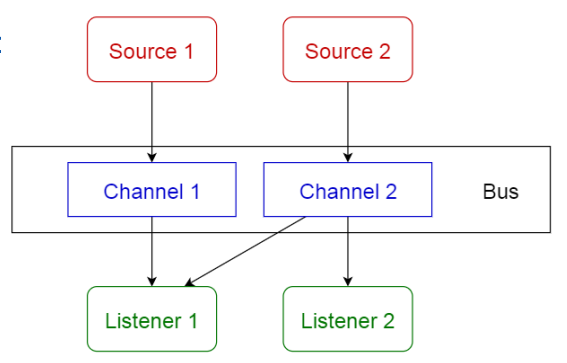
\includegraphics[width=0.3\textwidth] {Resources/Images/EventBus.png}
\caption{\label{fig:EventBus}EventBus}
\end{figure}

\end{multicols}

\pagebreak

\subsubsection{Model View Controller Pattern}

\begin{multicols}{2}
	\begin{itemize}
		\item Interaktive Anwendung in 3 Komponenten:
		\begin{itemize}
			\item \colorbox{violet!40} {Model:} Daten und Logik
			\item \colorbox{violet!40} {View:} Informationsanzeige
			\item \colorbox{violet!40} {Controller:} Verarbeitung der Benutzereingabe
		\end{itemize}
		\item Entkopllung UI und Logik
		\item Erlaubt Austauschbarkeit des UIs
		\item Alternativen:
		\begin{itemize}
			\item MVVM: Model View View Model
			\item MVP: Model View Presenter
		\end{itemize}
	\end{itemize}
\columnbreak

\begin{figure}[H]			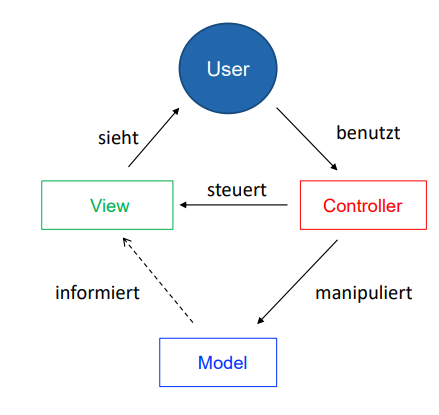
\includegraphics[width=0.3\textwidth] {Resources/Images/MVC.png}
\caption{\label{fig:MVC}MVC}
\end{figure}

\end{multicols}




















































\end{document}